\documentclass[a4paper,12pt]{article}
\usepackage[latin1]{inputenc}
\usepackage{ngermanb}
\usepackage[ngermanb]{babel}
\usepackage{graphicx}

\usepackage[noindentafter]{titlesec}
\usepackage[latin1]{inputenc}
\usepackage{ngermanb}
\usepackage[ngermanb]{babel}
\usepackage{graphicx}
\usepackage{url}
\usepackage{hyperref}
\usepackage[noindentafter]{titlesec}
\usepackage{vhistory}
\usepackage{pdflscape} 
\usepackage{listings}
% paragraphs sehen aus wie subsubsubsections
\titleformat{\paragraph}[hang]{\bf}{\thetitle\quad}{0pt}{}						
\titlespacing{\paragraph}{0pt}{1em}{0.5em} 

% subparagraphs sehen aus wie vorher paragraphs
\titleformat{\subparagraph}[runin]{\bf}{}{0.5em}{}
\titlespacing{\subparagraph}{0pt}{1em}{1em}



%opening
\title{Discrete Continous Response}
\author{Florian Hillen}

\begin{document}
\section{Discrete Continous Response}
This response is generated by convolution of the sampled continous Kernel with
the time-discrete difference equation.

\begin{figure}[htbp]
   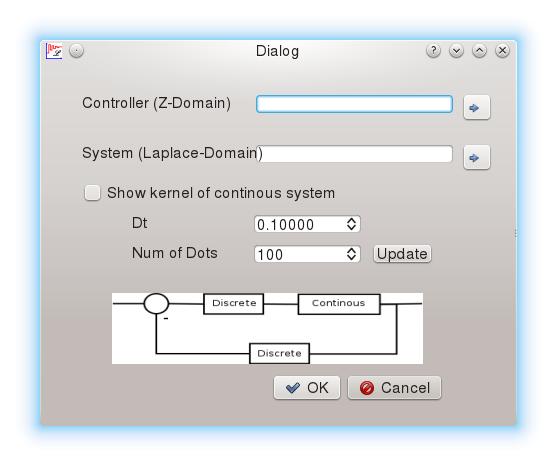
\includegraphics[width=350pt, keepaspectratio]{discretecontinous.png}
   \centering
 \caption{Discrete Continous System Dialog}
\label{PROCESSDIA}
\end{figure}
The equation for the discrete Controller has to be in it's Z-Form with the
complex variable named z. The continous transferfunction of the system has to
be in laplace-Form with the complex variable named s.
With the buttons on the left hand side of the expression's one has access to a
user defined library of expressions. Also the named Expressions in the side-panel
can be referenced.




\end{document}
